% !TEX root = ./physics.tex

\chapter{Module 5 \; Advanced Mechanics}

\section{Practical Investigation 5.1}
	Aim: To confirm the dependence of the range of a projectile (the horizontal distance it travels) on its time of flight and launch velocity by predicting the landing point of a projectile and then testing the prediction.

	\subsection{Variables}
	\begin{table}[htbp]
		\centering
		\begin{tabular}{l|l|l}
			Independent & Dependent & Controlled \\ \hline
			Height of drop 	& Initial velocity 	& Angle of ramp \\
			 				& Range 			& Distance of flat surface \\
			 				& 					& Acceleration due to gravity \\
			 				& 					& Type and size of ball \\ 
		\end{tabular}
	\end{table}

	\subsection{Materials}
	\begin{enumerate}
		\item Ball
		\item Inclined plane
		\item Pen
		\item Stopwatch
		\item Ruler
	\end{enumerate}

	\subsection{Method}
		\begin{enumerate}
			\item Prepare a ramp facing the edge of the table, 50 cm away.
			\item Mark 5 cm intervals along ramp
			\item Release ball at an interval
			\item Record time taken to travel 50cm flat distance and distance from table after drop
			\item Repeat steps 3-4 for each interval 3 times.
			\item Calculate the initial velocity of the drop using v = delta s/delta t
			\item Calculate the time of flight using height of table ($height=\frac{1}{2}\times (-9.8)t^2$), hence estimate the horizontal range of the ball ($s_{x} = ut$)
			\item Graph estimated range and actual range over velocity and compare.
		\end{enumerate}

	\subsection{Results}
		\begin{figure}[H]
			\centering
			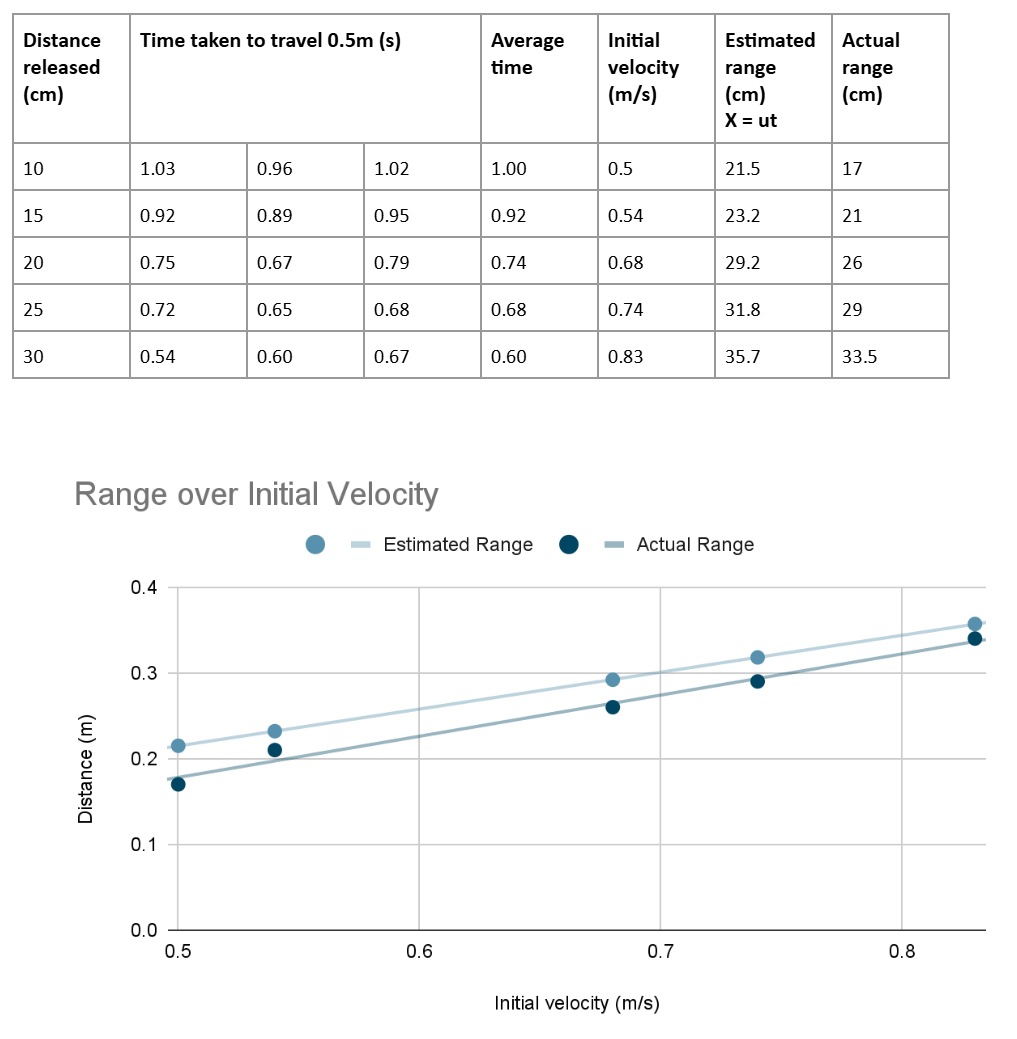
\includegraphics[width=15cm]{prac 5.1 table of results.png}
		\end{figure}

	\subsection{Data and Analysis}
		\subsubsection{Part A}
			Distance across tabletop: 0.5m
			\begin{enumerate}
				\item \textbf{Is the velocity being calculated the velocity of the ball at the edge of the table? If not, is it a reasonable approximation? Explain your answer.}
					\subitem Although the calculated velocity is not completely accurate due to friction forces, it is a reasonable approximation when assuming friction is minimal.
				\item \textbf{What effect would increasing the horizontal distance have on the reliability of your measurements?}
					\subitem Increasing the distance would make the experiment more reliable at the cost of accuracy.
			\end{enumerate}

		\subsubsection{Part B}
			Height above the ground: 0.90m
			\begin{enumerate}
				\item \textbf{Calculate the time it takes for the ball to fall from the table to the floor.}
					\begin{align}
						s &= ut + \frac{1}{2}at^2 \\
						0.9 &= (0)t + \frac{1}{2}(-9.8)t^2 \\
						t^2 &= \frac{2 \times 0.9}{9.8} \\
						t &= \sqrt{\frac{2 \times 0.9}{9.8}} \\
						&= 0.43 s
					\end{align} 
				\item \textbf{Calculate the distance the ball will travel in the horizontal direction, ie. the range}
					\begin{align*}
						s &= ut + \frac{1}{2}at^2 \\
						&= u(0.43) + \frac{1}{2}(0)(0.43)^2\\
						&= 0.43u
					\end{align*}
			\end{enumerate}

	\subsection{Discussion}
		Controlled variables were somewhat maintained to provide validity to the experiment, however numerous sources of error arose. Sources of error included:
		\begin{itemize}
			\item Ramp moving after ball was placed
			\item Irregular ball movements due to variations in placement and imperfections of ramp
			\item Inconsistency of measurement of horizontal range
			\item Timing of ball over flat distance
		\end{itemize}
		These errors were mitigated, however could not be avoided. The experiment was repeated three times for each interval to reduce the effect of outliers. More tests per interval could have been conducted to improve the reliability.
	
	\subsection{Conclusion}
		\begin{enumerate}
			\item \textbf{State whether your prediction was successful, and describe any difficulties encountered in testing the prediction.}
				\subitem The prediction was successful, with a small but consistent variation from the expected value.
			\item \textbf{In this experiment, the assumption was made that there is negligible effect from air resistance. Would the effect of air resistance be more significant if the ball was released from a height of 30 cm up the ramp or 15 cm? Explain.}
				\subitem If released from a higher point, the effect of air resistance would be more significant as there are more air particles applying friction forces to the ball. However, the effect of this resistance would still be minimal.
			\item \textbf{What is the major source of error in this experiment? What steps were taken to minimise it?}
				\subitem The major source of error in this experiment is the human variation when timing with the stopwatch. This was mitigated by using slow motion cameras to more accurately measure the time taken for the ball to travel across the flat surface.
		\end{enumerate}


\section{Practical Investigation 5.2 - The effect of launch angle on range}

	Aim: To investigate the relationship between the launch angle of a projectile, its motion and the range of the projectile. \;

90cm vertical height
	\subsection{Method}
		\begin{enumerate}
			\item Set the launcher in the horizontal position with a launch angle of 0\textdegree.
			\item Load a projectile into the launcher and ensure that the launcher is set to its maximum compression or distance setting.
			\item Launch the projectile, and note the point of impact on the paper.
			\item Lay a sheet of carbon paper on top of the white paper over the point of impact, carbon side down, so that when a ball lands on it there will be a mark on the paper.
			\item Place a sheet of paper where the ball hits. Highlight the point with a pencil or marker when the projectile lands.
			\item State recording with the data collection system and launch the projectile
			\item Use the angle indicator on the launcher the angle of inclination by 10\textdegree each time for data points between 10\textdegree and 80\textdegree.
			\item Measure the horizontal velocity for each angle.
		\end{enumerate}

	\subsection{Results}
		\begin{table}[htbp] \label{5.2 Table of Results}
			\centering
			\begin{tabular}{l|l|l}
				Angle (\textdegree) & Time (s)	& Horizontal Range (m)  \\ \hline
				0 					& 0.46		& 1.5 		\\
				0 					& 0.41		& 1.65		\\ \hline
				10					& 0.46		& 1.94		\\
				10					& 0.61		& 2.00		\\
				10					& 0.59		& 1.85		\\ \hline
				20					& 0.61		& 2.03		\\
				20					& 0.65		& 1.98		\\
				20					& 0.58		& 2.003		\\ \hline
				30					& 0.83		& 2.065		\\
				30					& 0.71		& 2.122		\\
				30					& 0.83		& 2.185		\\ \hline
				40					& 0.79		& 2.22		\\
				40					& 0.70		& 2.16		\\
				40					& 0.78		& 2.14		\\ \hline
				50					& 0.85		& 1.99		\\
				50					& 0.83		& 1.845		\\
				50					& 0.93		& 2.031		\\ \hline
				60					& 0.96		& 1.708		\\
				60					& 0.85		& 1.76		\\
				60					& 0.88		& 1.59		\\ \hline
				70					& 0.85		& 1.14		\\
				70					& 0.83		& 1.21		\\
				70					& 0.86		& 1.31		\\ \bottomrule
			\end{tabular}
		\end{table}

		\begin{table}[htbp]
			\centering
			  \begin{tabular}{lllllllll}
			  Angle \textdegree & \multicolumn{4}{l}{Time (s)}      & \multicolumn{3}{l}{Horizontal Range (m)} &  \\
					& Trial 1 & T2    & T3    & \textbf{Avg} & Trial 1 & 2     & 3     & \textbf{Avg} \\
			  0     & 0.46  & 0.41  &       & \textbf{0.44} & 1.50  & 1.65  &       & \textbf{1.58} \\
			  10    & 0.46  & 0.61  & 0.59  & \textbf{0.55} & 1.94  & 2.00  & 1.85  & \textbf{1.93} \\
			  20    & 0.61  & 0.65  & 0.58  & \textbf{0.61} & 2.03  & 1.98  & 2.00  & \textbf{2.00} \\
			  30    & 0.83  & 0.71  & 0.83  & \textbf{0.79} & 2.07  & 2.12  & 2.19  & \textbf{2.12} \\
			  40    & 0.79  & 0.70  & 0.78  & \textbf{0.76} & 2.22  & 2.16  & 2.14  & \textbf{2.17} \\
			  50    & 0.85  & 0.83  & 0.93  & \textbf{0.87} & 1.99  & 1.85  & 2.03  & \textbf{1.96} \\
			  60    & 0.96  & 0.85  & 0.88  & \textbf{0.90} & 1.708 & 1.76  & 1.59  & \textbf{1.69} \\
			  70    & 0.85  & 0.83  & 0.86  & \textbf{0.85} & 1.14  & 1.21  & 1.31  & \textbf{1.22} \\
			  \end{tabular}
		\end{table}

		\begin{figure}[H]
			\centering
			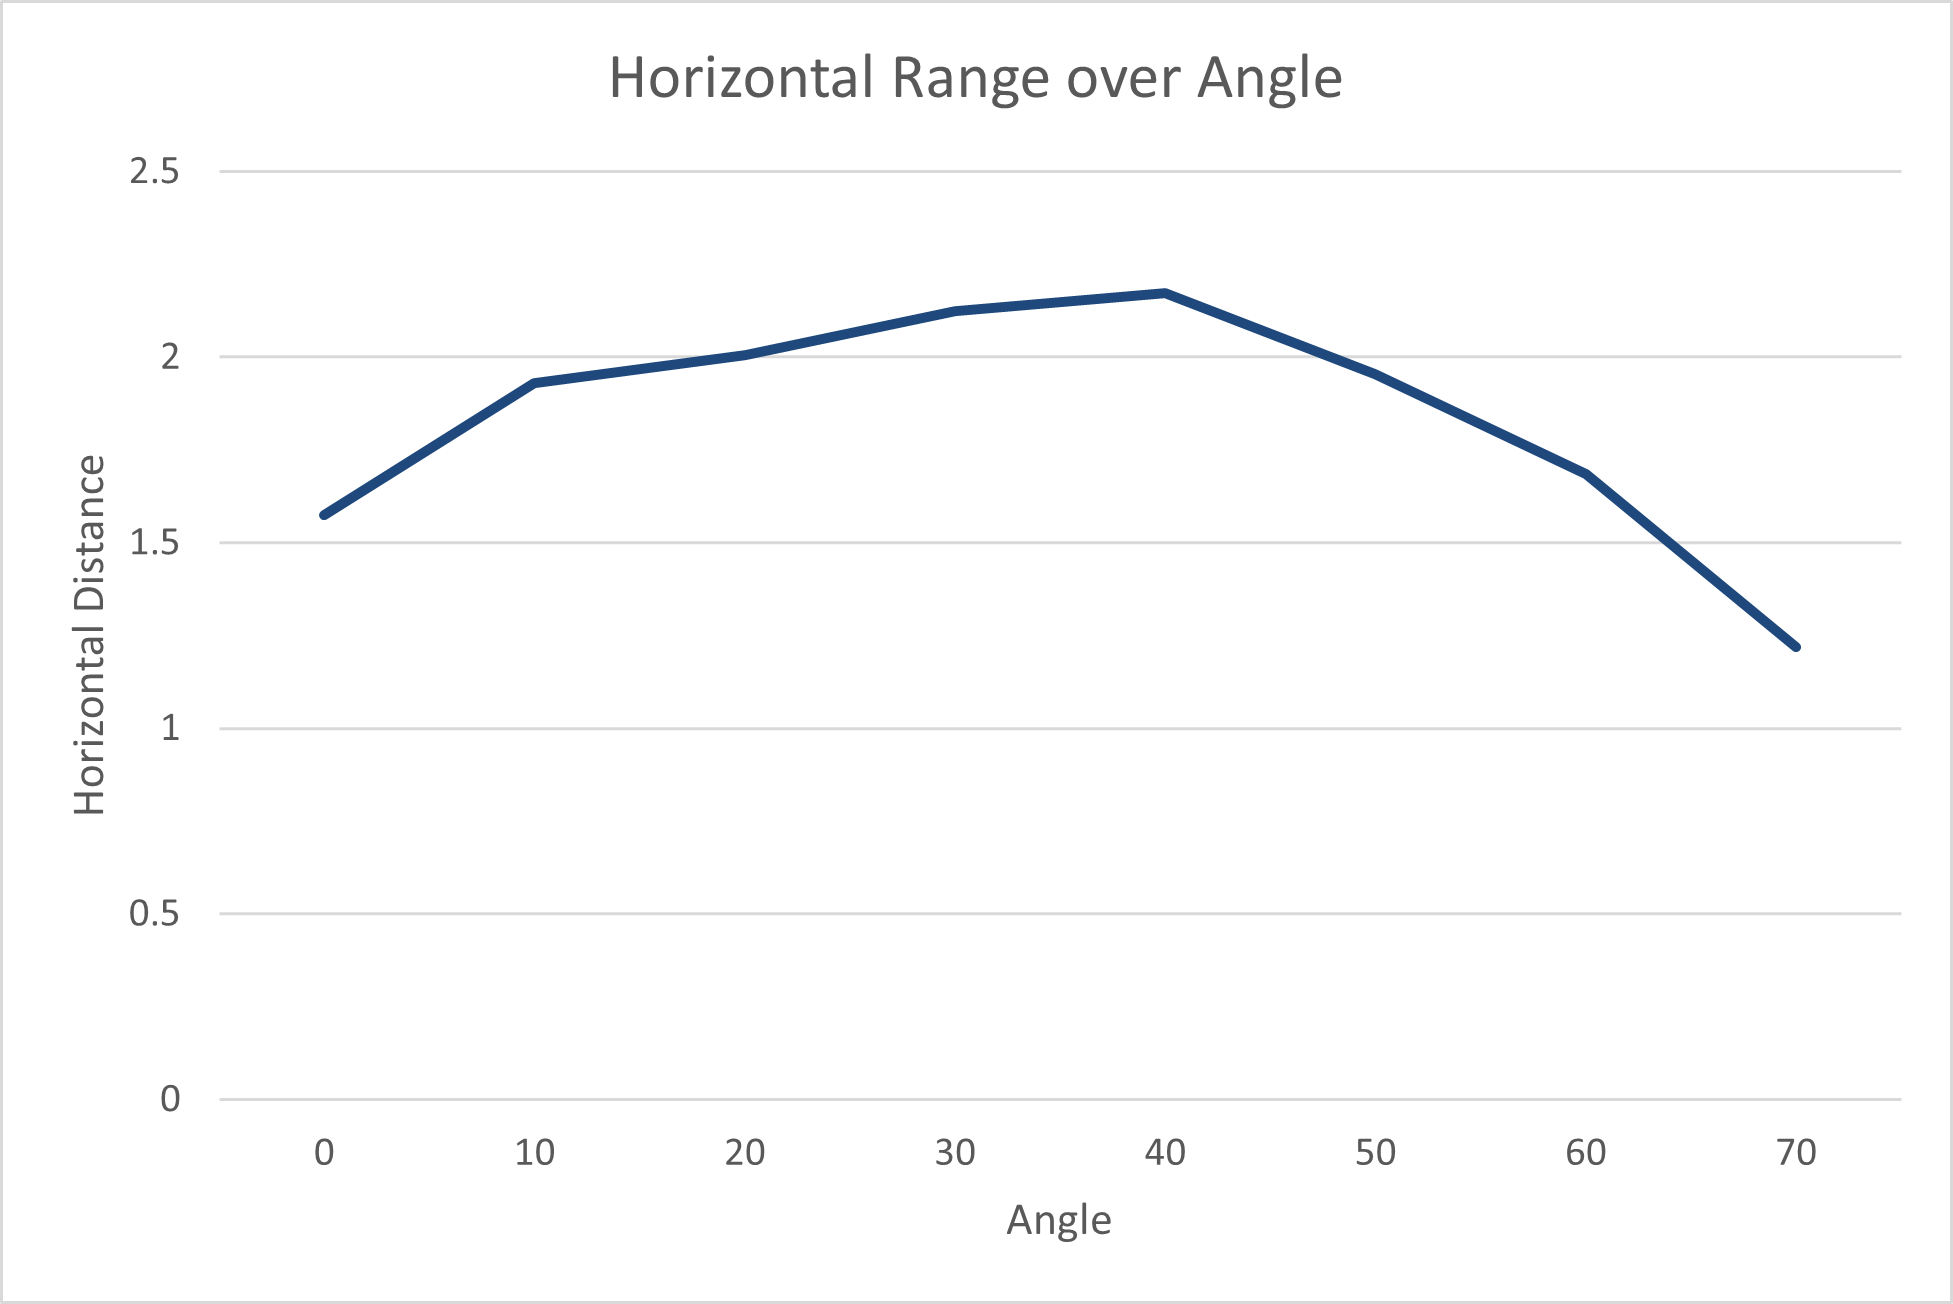
\includegraphics[width=15cm]{prac 5.2 horiz range over angle.png}
		\end{figure}

	\subsection{Conclusion}
		\begin{enumerate}
			\item \textbf{How did the measured horizontal velocities compare to the average horizontal velocities?}
				\subitem The measured horizontal velocities were similar to the average horizontal velocities.
			\item \textbf{For any projectile launched horizontally, what can you state about the horizontal velocity?}
				\subitem The horizontal velocity will be constant throughout the time of flight
			\item \textbf{Which launch angle will yield the maximum range?}
			\item \textbf{Which launch angle will yield the maximum range?}
				\subitem 40\textdegree
			\item \textbf{Are there launch angles that yield the same range? What are they and why is that the case?}
				\subitem There are some launch angles that yield the same range. This is due to the parabolic shape of the range versus angle graph, meaning that there are two points on either side of the ideal (40\textdegree) that provide the same range.
		\end{enumerate}

\section{Circular Motion} \label{4/11/2024}
	\subsection{Uniform Circular Motion}
	Occurs when objects travel in a circle at a constant speed, taking the same length of time to make each revolution

	The period T is the time taken to travel the full circle

	The distance covered during the period depends upon the radius of the circle of travel and is equal to the circle's circumference, ie. $d=2\pi r$

\section{Practical Investigation 5.3 - Circular Motion - centripetal force in a horizontal plane}

	Aim: To investigate the relationship between the centripetal force acting on an object moving in a circle of constant radius and the frequency of revolution.
	Aim: To investigate the relationship between the centripetal force acting on an object moving in a circle of constant radius and the frequency of revolution.

	\subsection{Method}
		\begin{enumerate}
			\item Securely tie one end of the fishing line to the small, soft mass
			\item Pass the fishing line down through the thin plastic tube and attach a 50g slotted mass carrier to the end.
			\item Attach an alligator clip to the line to act as a marker for a measured radius of around 1 m.
			\item Spin the stopper in a horizontal circular path at a speed that pulls the paperclip up to, but not touching the bottom of the tube.
			\item Measure time taken for 20 revolutions
			\item Add 50g and repeat steps.
		\end{enumerate}

		\begin{table}[htbp]
			\centering
			\begin{tabular}{llllllllll}
			Mass (kg) & \multicolumn{4}{c}{Time for 20 revolutions (s)} & \multicolumn{1}{l}{Period (s)} & \multicolumn{1}{l}{f=1/T} & \multicolumn{1}{l}{$F_c$ (N)} & \multicolumn{1}{l}{$F_G$ (N)} & \multicolumn{1}{l}{$\omega$ \textdegree$s^{-1}$} \\
					& \multicolumn{1}{l}{Trial 1} & 2     & 3     & \multicolumn{1}{l}{Avg} &       &       &       &       &  \\ \hline
			\multicolumn{1}{r}{0.05} & 10.34 & 10.78 & 12.34 & 11.15 & 0.558 & 1.79  & 0.6601 & 0.49  & 11.27 \\
			\multicolumn{1}{r}{0.1} & 9.00  & 8.97  & 8.85  & 8.94  & 0.447 & 2.24  & 1.027 & 0.98  & 14.06 \\
			\multicolumn{1}{r}{0.15} & 7.93  & 7.22  & 7.25  & 7.47  & 0.373 & 2.68  & 1.473 & 1.47  & 16.83 \\
			\multicolumn{1}{r}{0.2} & 6.56  & 6.47  & 7.03  & 6.69  & 0.334 & 2.99  & 1.837 & 1.96  & 18.79 \\
			\end{tabular}
		\end{table}
		
	\subsection{Data and Analysis}
		Measured radius of revolution: 0.5m
		\begin{enumerate}
			\item \textbf{What force is the mass carrier providing in this experiment}
				\subitem The mass carrier is exerting a gravitational force on the string
		\end{enumerate}

		\begin{figure}[H]
			\centering
			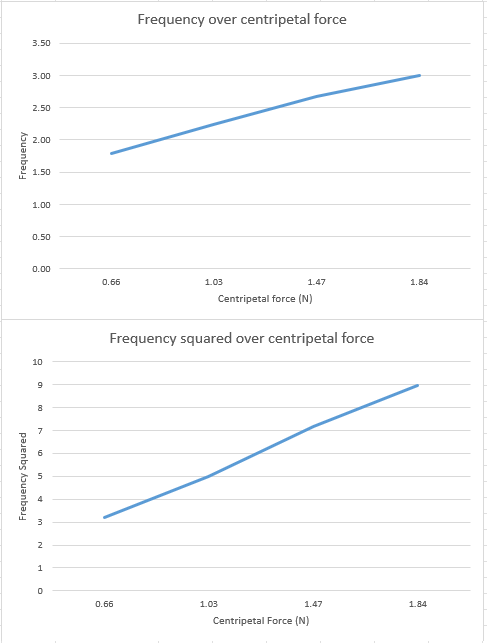
\includegraphics[width=8cm]{5.3 graphs.png}
		\end{figure}

	\subsection{Conclusion}
		\begin{enumerate}
			\item \textbf{Based on your results, what is the relationship between the centripetal force and the frequency of rotation? Do your results confirm what was expected from theory? Comment on any differences.}
				\subitem Based on the results, centripetal force has an square root graph relationship to frequency of rotation. This is expected, as $F_{c}=\frac{mv^2}{r}$, with velocity being squared.
			\item \textbf{The radius of revolution will not actually be quite what was measured, nor will the tension in the string be exactly equal to the centripetal force. Why is this so?}
				\subitem Due to human inaccuracies, the radius of revolution will vary as the mass moves up and down. It is difficult to maintain a set tension, so this variation is expected. Because of this, the tension will also not be equal to the weight force applied by the mass.
			\item \textbf{What effect does this have on your results}
				\subitem This will shift the results slightly away from the expected value, but each factor somewhat counteracts the other so this is minimised.
		\end{enumerate}

\section{Types of Centripetal Force} \label{11/11/2024}
	Centripetal force is not a fundamental force, rather a label given to the net force that causes an object to move in a circular path. Centripetal force can occur due to:
	Centripetal force is not a fundamental force, rather a label given to the net force that causes an object to move in a circular path. Centripetal force can occur due to:
	\begin{itemize}
		\item Friction
		\item Banking (Reaction force at an angle)
		\item Tension
		\item Gravity
		\item Magnetic force
		\item Electrostatic force
	\end{itemize}

	\subsection{Centripetal Force by Friction}
		Sideways (lateral) friction between the tyres and the road opposes the inertial outward (tangential) motion, acting inwards towards the centre of the curve.

		As this sideways friction makes up the magnitude of the net force, it is the centripetal force that keeps the car moving around the curve.

		$$F_{net} = F_f = \mu N$$

		$$F_c = \mu N = \mu (-W) = \frac{mv^2}{r}$$

		\textbf{Sample Problem}

		A 1200 kg car approaches a tight corner on a wet day. If the corner has a radius of curvature of 10 m and the coefficient of friction of the tyres on the wet road is 0.4, what is the maximum speed at which the car can safely turn the corner?

		$$m = 1200\;\text{kg},\; r = 10\;\text{m},\;\mu = 0.4,\; F_{c} = ?$$

		\begin{align*}
			W &= mg = (1200)(9.8) = 11800\;\text{N downwards} \\
			R &= -W = -11800\;\text{N upwards}
		\end{align*}

		\begin{align*}
			F_{f} &= \mu R \\
			&= (0.4)(11800) \\
			&= 4720\;\text{N inwards towards the centre of the corner}
		\end{align*}

		The centripetal force must not exceed the frictional force if the car is to corner safely, therefore:
		\begin{align*}
			F_f &\ge F_c \\
			F_f &\ge \frac{mv^2}{r} \\
			4720 &\ge \frac{1200 \times v^2}{10} \\
			v &\le \sqrt{\frac{4720 \times 10}{1200}} \\
			v &\le 6.2ms^{-1} \\
		\end{align*}
		Therefore, the car can turn less than than 6.3 m/s (23 km/h)

	\subsection{Centripetal Force by Reaction Force}
		If the object undergoing centripetal motion is leaning at an angle, the normal reaction force needs to be dissected into vertical and horizontal components.

		The perpendicular component ($R_{\perp}$) is equal and opposite to the weight force ($W$)

		$$R_{\perp} = -W = 0$$

		$F_{net}$ is the parallel component of the normal reaction force

		$$R_{\parallel} = R \sin{\theta}$$
	
	\subsection{Centripetal Force by Banking}
		The angling of a surface that an object is moving in a circular motion maximises the speed at which the object can move.

		$$F_{net} = R\sin{\theta} + F_{f}\cos{\theta}$$

		The net force acting horizontally towards the centre of the curve is the sum of the horizontal components of the normal reaction force $R_R$ and the frictional force $F_f$.

	\subsection{Centripetal Force by Tension}
		\begin{align*}
			F_{net} &= F_c \\
			&= T + W
		\end{align*}
		Resolving the horizontal component:
		\begin{align*}
			\theta &= \arccos{\frac{F_{net}}{T}} \\
			F_{net} &= T\cos{\theta}
		\end{align*}
		Resolving the vertical component:
		\begin{align*}
			\theta &= \arcsin{\frac{W}{T}} \\
			W &= T\sin{\theta}
		\end{align*}
		\begin{figure}
			\centering
			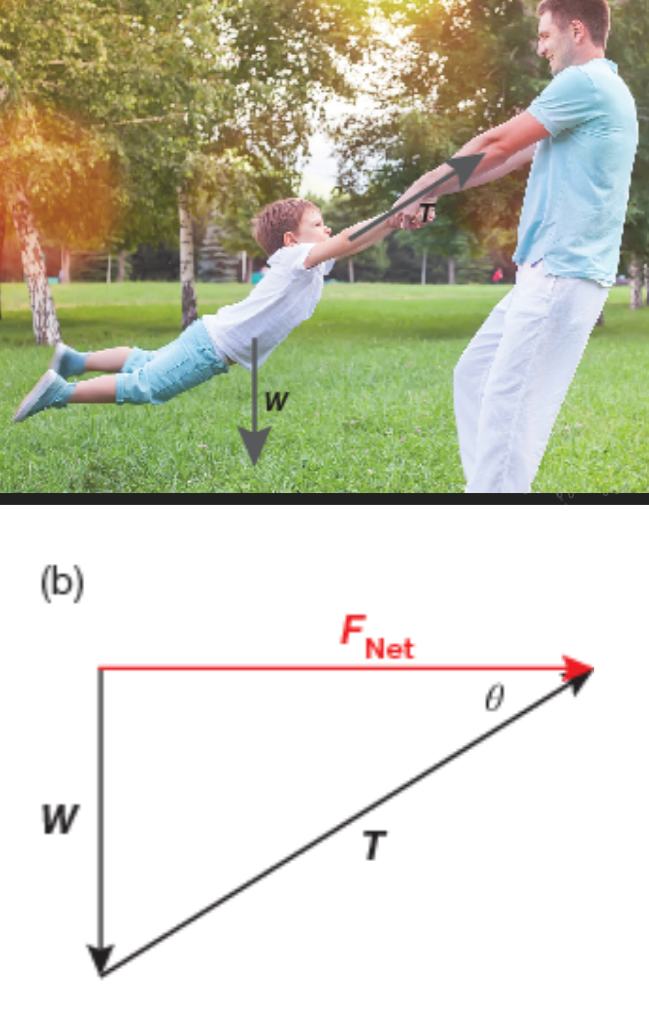
\includegraphics[height=8cm]{tension diagram.png}
		\end{figure}

	\subsection{Conical Pendulum}
		Tension force of the pendulum provides centripetal force

		$$F_c = T\sin{\theta} = \frac{mc^2}{r}$$

		The radius can be calculated from the length of the pendulum:

		$$r=l\sin{\theta}$$
		

\section{Practical Investigation 5.4 - Centripetal force in a vertical plane} \label{13/11/2024}
	
	Aim: To investigate the non-uniform nature of the forces acting in vertical circular motion\S
	
	\subsubsection{Notes}
	\begin{itemize}
		\item Mass of weight was 10.4g
	\end{itemize}

	\subsection{Method}
		\begin{enumerate}
			\item Tie the string to the mass and measure the length of the string to the centre of the mass. Mark the string in 10 cm segments.
			\item Use an alligator clip to mark a point and reduce friction when spinning.
			\item Rotate the mass in a vertical circle. Keep rotation as even as possible.
			\item Time the period of rotation for 20 revolutions and then find the average period. Repeat 3 times for each radius.
		\end{enumerate}

	\subsection{Results}
		\begin{table}[htbp]
			\centering
			  \begin{tabular}{l|lll|l|lll|l}
			  \multicolumn{1}{c}{Radius (m)} & \multicolumn{4}{c}{Time for 20 Revolutions (s)} & \multicolumn{3}{c}{Period T for one revolution} & \multicolumn{1}{c}{$T_{av}$} \\[5pt] \hline
					& Trial 1 & Trial 2 & Trial 3 & \textbf{Average} & Trial 1 & Trial 2 & Trial 3 & \textbf{Average} \\
			  0.1   & 6.63  & 6.78  & 6.25  & 6.55  & 0.33  & 0.34  & 0.31  & 0.33 \\
			  0.2   & 9.04  & 9.19  & 9.06  & 9.10  & 0.45  & 0.46  & 0.45  & 0.45 \\
			  0.3   & 12.00 & 11.44 & 11.82 & 11.75 & 0.60  & 0.57  & 0.59  & 0.59 \\
			  0.4   & 13.66 & 14.34 & 14.00 & 14.00 & 0.68  & 0.72  & 0.70  & 0.70 \\
			  0.5   & 17.10 & 16.50 & 16.91 & 16.84 & 0.86  & 0.83  & 0.85  & 0.84 \\
			  0.6   & 19.13 & 19.50 & 19.18 & 19.27 & 0.96  & 0.98  & 0.96  & 0.96 \\
			\end{tabular}
		\end{table}
		
		\begin{figure}[H]
			\centering
			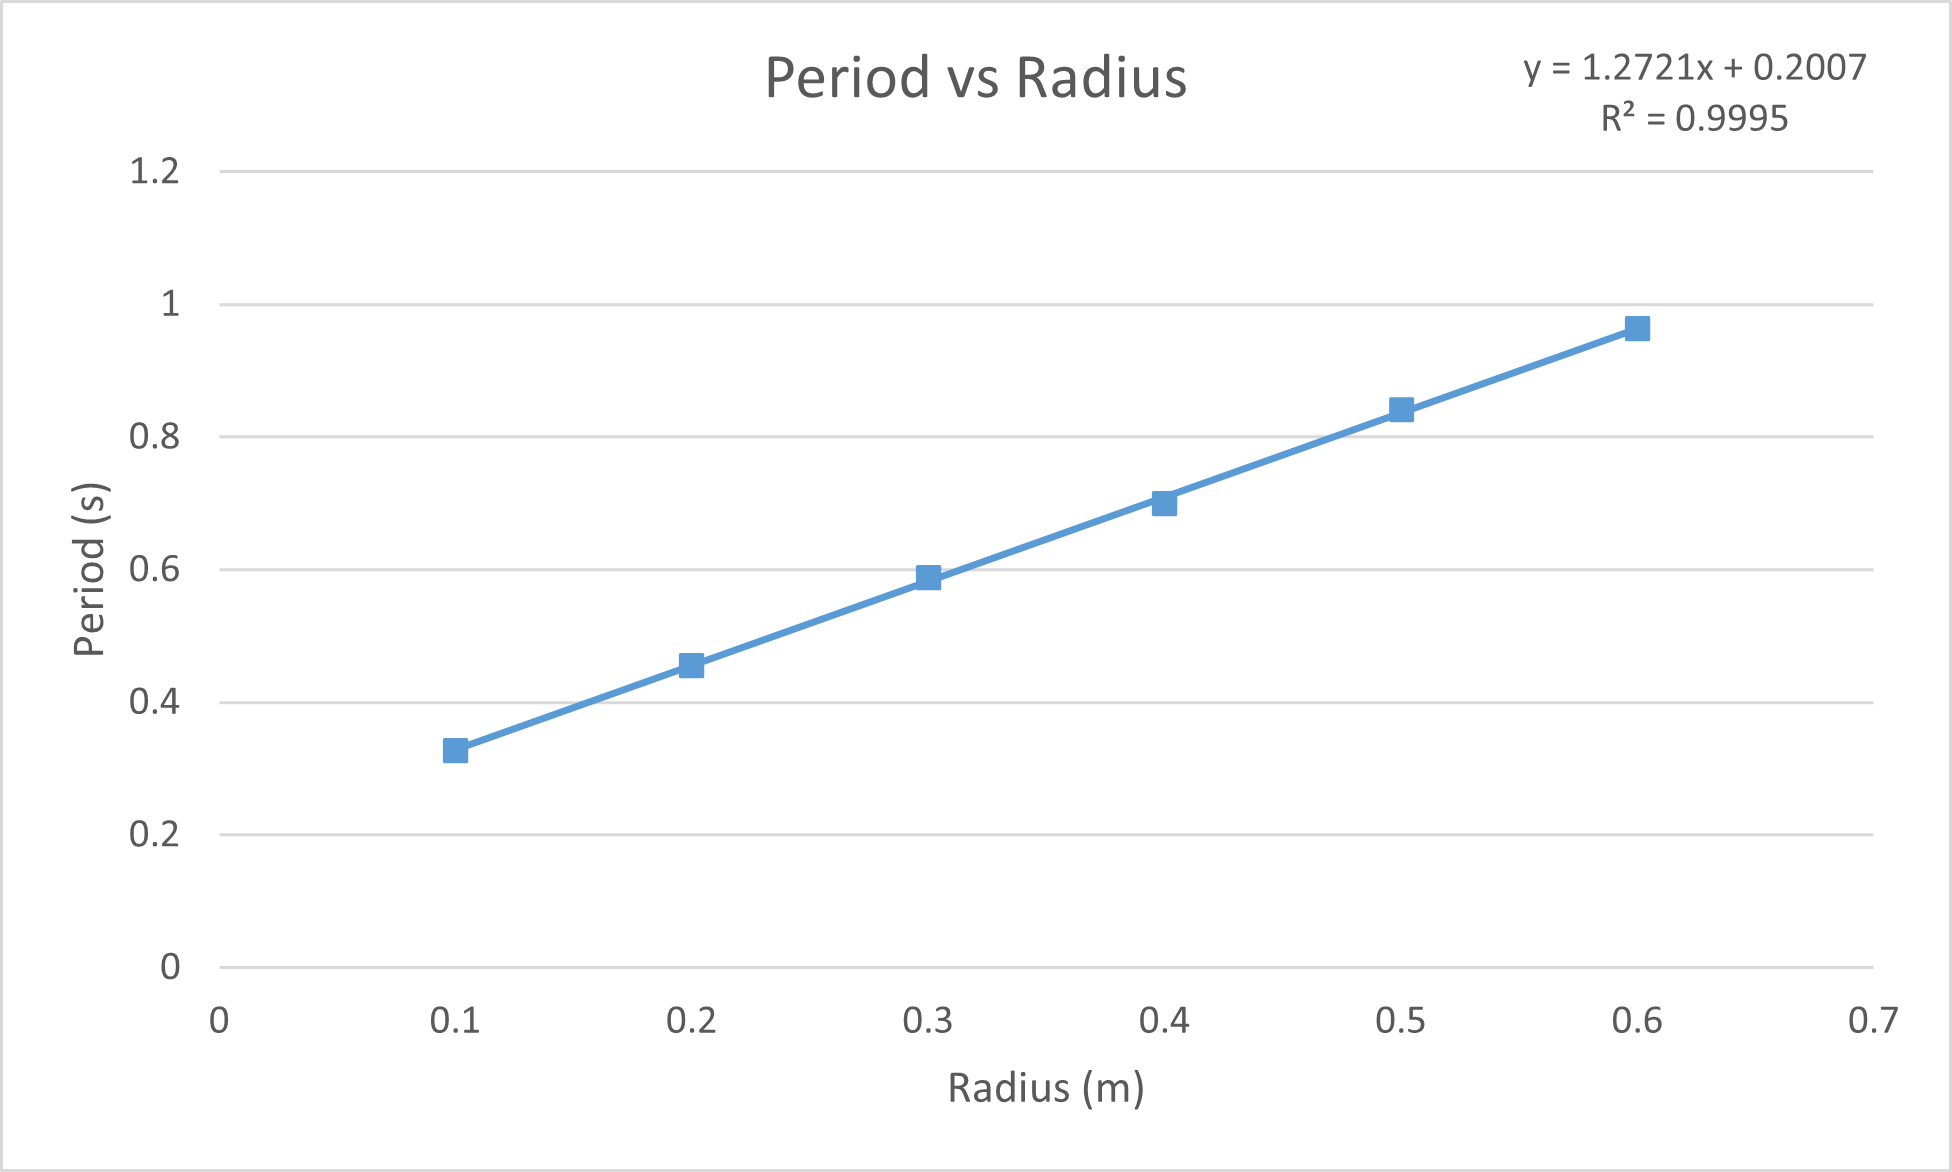
\includegraphics[width=15cm]{5.4 Period over radius graph.png}
		\end{figure}

	\subsection{Conclusion}
<<<<<<< Updated upstream
		\textbf{Based on your graph, comment on the relationship between period and radius. Do your results confirm what was expected from theory? Comment on any discrepancies}
		There is a linear relationship between period and radius
=======
	\begin{enumerate}
		\item \textbf{Why is a graph of period versus radius being plotted?}
			\subitem A graph is being plotted to show the effect of radius on period.
		\item \textbf{Based on your graph, comment on the relationship between period and radius. Do your results confirm what was expected from theory? Comment on any discrepancies}
			\subitem There is a linear relationship between period and radius.
	\end{enumerate}

\section{Angular Velocity} \label{18/11/2024}
